\documentclass[border=0.2cm]{standalone}

% More defined colors
\usepackage[dvipsnames]{xcolor}

% Required package
\usepackage{tikz}
\usetikzlibrary{positioning, calc}
\usetikzlibrary{shapes.geometric, ,decorations.markings}

% Bus diagonal lines: https://tex.stackexchange.com/questions/125460/drawing-bus-width-like-markers-with-number-on-arrows?noredirect=1&lq=1

\tikzset{
	multiplexer/.style={
		draw,
		trapezium,
		shape border uses incircle, 
		shape border rotate=270,
		minimum size=18pt
	}  
}

\begin{document}
	
	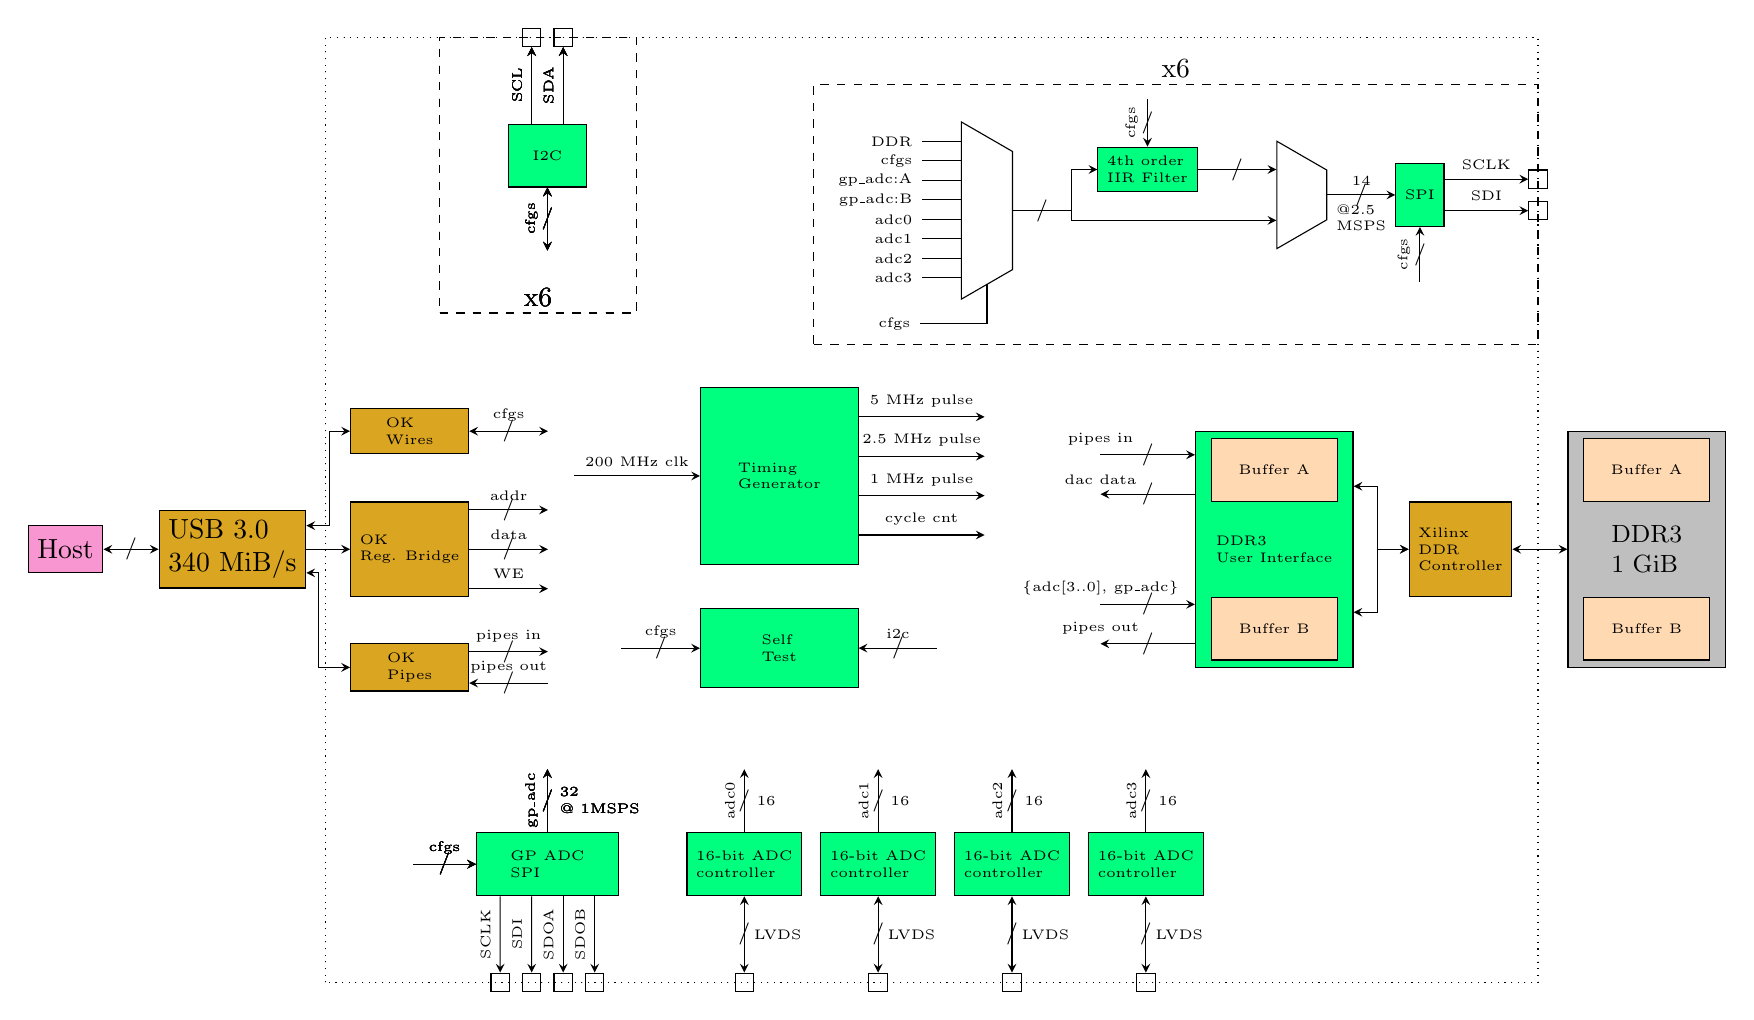
\begin{tikzpicture}[
		decoration={
			markings,
			mark= at position 0.5 with {\node[font=\footnotesize] {/};}
		}]
		
		
		\node[draw,
		minimum size=0.6cm,
		fill=Rhodamine!50
		] (host) at (0,0){Host};
		
		% USB connection
		\node [draw,
		fill=Goldenrod,
		align=left,
		right=0.7cm of host
		]  (usb) {USB 3.0 \\ $340$ MiB/s};

		% OpalKelly Wires
		\node [draw,
		fill=Goldenrod,
		align=left,
		minimum width=1.5cm, 
		on grid,
		above right=1.5cm and 2.25cm of usb,
		font=\tiny]  (wires) {OK \\ Wires};
		\draw[stealth-stealth, postaction={decorate}] (wires.east) -- ++(1,0) 
		node[midway,above]{\tiny cfgs};

		% OpalKelly Register Bridge
		\node [draw,
		fill=Goldenrod,
		align=left,
		on grid,
		minimum height=1.2cm,
		minimum width=1.5cm, 
		below right=1.5cm and 0.0cm of wires,
		font=\tiny]  (regbridge) {OK \\ Reg. Bridge};
		\draw[-stealth, postaction={decorate}] ($(regbridge.east) + (0.0,+0.5)$) -- ++(1,0) 
		node[midway,above]{\tiny addr};
		\draw[-stealth, postaction={decorate}] ($(regbridge.east) + (0.0,0)$) -- ++(1,0) 
		node[midway,above]{\tiny data};
		\draw[-stealth] ($(regbridge.east) + (0.0,-0.5)$) -- ++(1,0) 
		node[midway,above]{\tiny WE};
	
		% OpalKelly Pipes
		\node [draw,
		fill=Goldenrod,
		align=left,
		on grid,
		minimum width=1.5cm, 
		below right=3cm and 0.0cm of wires,
		font=\tiny]  (pipes) {OK \\ Pipes};
		\draw[-stealth, postaction={decorate}] ($(pipes.east) + (0.0,0.2)$) -- ++(1,0) 
		node[midway,above]{\tiny pipes in};
		\draw[stealth-, postaction={decorate}] ($(pipes.east) + (0.0,-0.2)$) -- ++(1,0) 
		node[midway,above]{\tiny pipes out};
	
		% connect from USB to OK API blocks 
		\draw[stealth-stealth] ($(usb.east) + (0.0,0.3)$) -- ++(0.3,0) |- (wires.west) node[]{};	
		\draw[-stealth] ($(usb.east) + (0.0,0.0)$) -- ++(0.3,0) |- (regbridge.west) node[]{};	
		\draw[stealth-stealth] ($(usb.east) + (0.0,-0.3)$) -- ++(0.15,0) |- (pipes.west) node[]{};	
		
		\node [draw,
		align=left,
		fill=SpringGreen, 
		minimum height=2.25cm,
		minimum width=2cm,
		above right=-0.7cm and 5cm of usb,
		font=\tiny
		] (timing) {Timing \\ Generator};
		
		\draw[stealth-] ($(timing.west)$) -- ++(-1.6,0) node [midway, above, font=\tiny]{200 MHz clk};
		\draw[-stealth] ($(timing.east) + (0,0.75)$) -- ++(1.6,0) node [midway, above, font=\tiny]{5 MHz pulse};
		\draw[-stealth] ($(timing.east) + (0,.25)$) -- ++(1.6,0) node [midway, above, font=\tiny]{2.5 MHz pulse};
		\draw[-stealth] ($(timing.east) + (0,-0.25)$) -- ++(1.6,0) node [midway, above, font=\tiny]{1 MHz pulse};
		\draw[-stealth] ($(timing.east) + (0,-0.75)$) -- ++(1.6,0) node [midway, above, font=\tiny]{cycle cnt};
		
		\node [draw,
		align=left,
		fill=SpringGreen, 
		minimum height=1cm,
		minimum width=2cm,
		below right=0.25cm and 5cm of usb,
		font=\tiny
		] (test) {Self \\ Test};
		\draw[stealth-, postaction={decorate}] ($(test.west)$) -- ++(-1,0) node [midway, above, font=\tiny]{cfgs};
		\draw[stealth-, postaction={decorate}] ($(test.east)$) -- ++(1,0) node [midway, above, font=\tiny]{i2c};	
		
		% DDR
		\node [draw,
		align=left,
		fill=Goldenrod, 
		minimum height=1.2cm,
		right=14cm of usb,
		font=\tiny
		] (ddr-control) {Xilinx \\ DDR \\ Controller};
		
		\node [draw,
		align=left,
		fill=lightgray, 
		minimum width=2cm, 
		minimum height=3cm,
		right=0.7cm of ddr-control,
		font=\small
		] (ddr) {DDR3 \\ 1 GiB};		
		
		\node[draw,fill=orange!30,minimum width=1.6cm, 
		minimum height=0.8cm, font=\tiny] at ([yshift=-0.5cm]ddr.north){Buffer A};
		\node[draw,fill=orange!30,minimum width=1.6cm, 
		minimum height=0.8cm, font=\tiny] at ([yshift=0.5cm]ddr.south){Buffer B};
		
		\node [draw,
		align=left,
		fill=SpringGreen, 
		minimum width=2cm, 
		minimum height=3cm,
		left=0.7cm of ddr-control,
		font=\tiny
		] (ddr-ui) {DDR3 \\ User Interface};		
		
		\draw[stealth-stealth] ($(ddr-ui.east) + (0.0,0.8)$)  -- ++(0.3,0) |- (ddr-control.west) node[]{};	
		\draw[stealth-stealth] ($(ddr-ui.east) - (0.0,0.8)$)  -- ++(0.3,0) |- (ddr-control.west) node[]{};	
		
		\node[draw,fill=orange!30,minimum width=1.6cm, 
		minimum height=0.8cm, font=\tiny] at ([yshift=-0.5cm]ddr-ui.north){Buffer A};
		\node[draw,fill=orange!30,minimum width=1.6cm, 
		minimum height=0.8cm, font=\tiny] at ([yshift=0.5cm]ddr-ui.south){Buffer B};

		\draw[-stealth, font=\tiny, postaction={decorate}] ($(ddr-ui.west) + (0.0,0.7)$)  -- ++(-1.2,0) node[above]{dac data};	
		\draw[stealth-, font=\tiny, postaction={decorate}] ($(ddr-ui.west) + (0.0,1.2)$)  -- ++(-1.2,0) node[above]{pipes in};	

		\draw[stealth-, font=\tiny, postaction={decorate}] ($(ddr-ui.west) + (0.0,-0.7)$)  -- ++(-1.2,0) node[above]{\{adc[3..0], gp\_adc\}};	
		\draw[-stealth, font=\tiny, postaction={decorate}] ($(ddr-ui.west) + (0.0,-1.2)$)  -- ++(-1.2,0) node[above]{pipes out};	


		\foreach \x [count=\xi] in {0,1,2,3} 
		{
			% ADC AD7961
			\node [draw,
			align=left,
			on grid,
			fill=SpringGreen, 
			minimum height=0.8cm,
			below right=4cm and 6.5cm+\x*1.7cm of usb,
			font=\tiny]  (adc\x) {16-bit ADC \\ controller};
			
			\node [draw,
			align=left,
			on grid,
			minimum width=0.1cm, 
			minimum height=0.1cm, 
			below right= 1.5cm and 0cm of adc\x
			]  (adcpad\x) {};
	
			\draw[stealth-stealth, postaction={decorate}] (adc\x.south) -- (adcpad\x.north) 
			node[midway,right]{\tiny LVDS};
			
			\draw[-stealth, postaction={decorate}] (adc\x.north)-- ++(0,0.8) 
			node[midway,above,rotate=90]{\tiny adc\x} 
			node[midway, right=1pt] {\tiny 16};
		}
		
		\node[multiplexer]
		(mul) at (15.7,4.5) {};

		\node [draw,
		align=left,
		on grid,
		minimum height=0.8cm, 
		fill=SpringGreen, 
		right=1.5cm of mul,
		font=\tiny
		] (spi) {SPI};		

		\draw[stealth-, postaction={decorate}] (spi.south)-- ++(-0,-0.7) 
		node[midway,above,font=\tiny, rotate=90]{cfgs};

		\node [draw,
		align=left,
		on grid,
		minimum width=0.1cm, 
		minimum height=0.1cm, 
		above right= 0.2cm and 1.5cm of spi
		]  (spipad1) {};
		
		\node [draw,
		align=left,
		on grid,
		minimum width=0.1cm, 
		minimum height=0.1cm, 
		above right= -0.2cm and 1.5cm of spi
		]  (spipad2) {};
		
		\draw[-stealth] ($(spi.east) + (0,0.2)$) -- (spipad1.west) 
		node[midway,above]{\tiny SCLK};
		\draw[-stealth] ($(spi.east) + (0,-0.2)$) -- (spipad2.west) 
		node[midway,above]{\tiny SDI};

		\draw[-stealth, postaction={decorate}] (mul.east) -- (spi.west) 
		node[midway,above, font=\tiny]{14}
		node[align=left, midway,below, font=\tiny]{@2.5 \\ MSPS};

		\node [draw,
		fill=SpringGreen,
		align=left,
		on grid,
		left=of mul.north west, anchor=east,
		font=\tiny
		]  (filter) {4th order \\ IIR Filter};
		
		\draw[stealth-, postaction={decorate}] (filter.north) -- ++(0,0.6) 
		node[midway,above,rotate=90,font=\tiny]{cfgs};
		
		\draw[-stealth, postaction={decorate}] (filter.east) -- (mul.north west) 
		node[midway,above]{};
		%\coordinate (muxl0) at ($(mul.south west)$); %($(muxl0) ++ (-3,0)$)
		\draw[]($(mul.south west) + (-4,-1)$) coordinate (O)--++(30:0.75)coordinate (A)--++(90:1.5)coordinate (B)--++(150:0.75)coordinate (C)--cycle;
		\draw[postaction={decorate}] ($(A)!0.5!(B)$)--++(0:0.75)node[right]{} coordinate (datamux);
		\draw[font=\tiny] ($(O)!0.5!(A)$)--++(-90:0.5)--++(180:0.85)node[left]{cfgs};

		\draw[-stealth] (datamux) |- (filter.west) 
		node[midway,above]{};
		\draw[-stealth] (datamux) |- (mul.south west) 
		node[midway,above]{};

		\foreach \y/\t in {0.1/DDR,0.2/cfgs,0.3/gp\_adc:A, 0.4/gp\_adc:B,0.5/adc0,0.6/adc1,0.7/adc2,0.8/adc3} {
			\draw[]  ($(C)! \y*1.1 !(O)$)--++(180:0.5) node[left] {\tiny \t};}
		
		\draw[stealth-stealth, postaction={decorate}] (host.east) -- (usb.west) 
		node[midway,above]{};
		\draw[stealth-stealth] (ddr-control.east) -- (ddr.west);
		
		\node (rect) at (14.1,4.25) [draw,dashed,minimum width=9.2cm,minimum height=3.3cm] []{};
		\node[] (right)  at ($(rect.north)+(0,0.2cm)$) {x6};
		
		% General purpose ADC SPI 
		\node [draw,
		align=left,
		on grid,
		minimum height=0.8cm, 
		minimum width=1.8cm, 
		fill=SpringGreen, 
		left=2.5cm of adc0,
		font=\tiny
		] (adcspi) {GP ADC \\ SPI};		
		
		\foreach \y/\t in {1/SCLK, 2/SDI, 3/SDOA,4/SDOB} {
		\node [draw,
		align=left,
		on grid,
		minimum width=0.1cm, 
		minimum height=0.1cm, 
		below right= 1.5cm and -1cm+\y*0.4cm of adcspi
		]  (adcspipad\y) {};
				
		\draw[-stealth] ($(adcspi.south) + (-1 + \y*0.4, 0)$) -- (adcspipad\y.north) 
		node[midway,above,rotate=90, font=\tiny]{\t};
		
		\draw[-stealth, postaction={decorate}] (adcspi.north)-- ++(0,0.8) 
		node[midway,above,rotate=90]{\tiny gp\_adc} 
		node[align=left, midway, right=1pt, font=\tiny] {32 \\ @ 1MSPS};

		\draw[stealth-, postaction={decorate}] (adcspi.west)-- ++(-0.8,0) 
		node[midway,above,font=\tiny]{cfgs};
		
		% I2C Controllers 
		\node [draw,
		align=left,
		on grid,
		minimum height=0.8cm, 
		minimum width=1cm, 
		fill=SpringGreen, 
		above=9cm of adcspi,
		font=\tiny
		] (i2c) {I2C};		
		
		\draw[stealth-stealth, postaction={decorate}] ($(i2c.south)$)  -- ++(0,-0.8) 
		node[midway,above,rotate=90, font=\tiny]{cfgs};
		
		\foreach \y/\t in {1/SCL, 2/SDA} {
			\node [draw,
			align=left,
			on grid,
			minimum width=0.1cm, 
			minimum height=0.1cm, 
			above right= 1.5cm and -0.6cm+\y*0.4cm of i2c
			]  (i2cpad\y) {};
			
			\draw[-stealth] ($(i2c.north) + (-0.6cm + \y*0.4cm, 0)$) -- (i2cpad\y.south) 
			node[midway,above,rotate=90, font=\tiny]{\t};
		}

	\node (i2cbox) at (6,4.75) [draw,dashed,minimum width=2.5cm,minimum height=3.5cm] []{};
	\node[] (right)  at ($(i2cbox.south)+(0,0.2cm)$) {x6};
	
	
	% FPGA outline
	\draw[dotted] (3.3,-5.5) rectangle (18.7, 6.5);
	
	}
		
	\end{tikzpicture}
	
\end{document}